\documentclass[10pt]{beamer}

\usepackage{fontspec}
\usepackage{xunicode}
\usepackage{xltxtra}
\setsansfont{FreeSans}
\setmonofont{DejaVuSansMono}

\usepackage{listings}
\usepackage{textpos}
\usepackage{tikz}
\usepackage{minted}

\setbeamertemplate{footline}[frame]
\setbeamertemplate{items}[default]
\usetheme{Warsaw}
\usecolortheme{seahorse}
\setbeamertemplate{itemize items}[default]
\setbeamertemplate{navigation symbols}{}
\setbeamertemplate{footline}[frame number]
\lstset{columns=fixed}
\setbeamerfont*{block body}{series=\tt}
\definecolor{lightgray}{rgb}{0.9,0.9,0.9}
\definecolor{midgray}{rgb}{0.5,0.5,0.5}

\usetikzlibrary{arrows,positioning,fit,backgrounds}
\tikzset{
    %Define standard arrow tip
    >=stealth',
    %Define style for boxes
    punkt/.style={
           rectangle,
           rounded corners,
           draw=black, very thick,
           text width=6.5em,
           minimum height=2em,
           text centered},
    % Define arrow style
    pil/.style={
           ->,
           thick,
           shorten <=2pt,
           shorten >=2pt,}
}

\newcommand{\light}[1]{\textcolor{gray}{\footnotesize{#1}}}
\newcommand{\code}[4]{\inputminted[linenos, frame=none, firstline=#2, lastline=#3,
  framesep=10pt, bgcolor=lightgray]{#4}{#1}}

\title[Bayecho]{Про ДНК, исправление ошибок и Echo}
\author{Дмитрий Грошев\\
  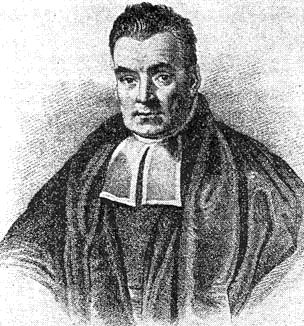
\includegraphics[height=3cm]{thomas_bayes.png}}
\date{26.10.2012}
\institute{СПбГУ}

\begin{document}
\renewcommand*{\inserttotalframenumber}{\pageref{lastframe}}
\begin{frame}
\titlepage
\end{frame}

%% Intro

\begin{frame}
  \begin{center}
    \Large
    Общие понятия
  \end{center}
\end{frame}

\begin{frame}{ДНК}
  \begin{itemize}
  \item ...ACGGGCACACTTACG...
  \item 4 нуклеотида: аденин, тимин, цитозин, гуанин (но это неважно)
  \item ДНК → РНК → белки → жизнь
  \item 4 миллиарда нуклеотидов у человека, ~4Gb данных
  \end{itemize}
\end{frame}

\begin{frame}{Секвенирование}
  \begin{itemize}
  \item чтение последовательности ДНК
  \item текущая технология — прочтение случайных участков по 100
  \item хорошее покрытие — 30+ (4Gb→120Gb)
  \item очень сложно собирать
  \item неидеальное прочтение
  \end{itemize}
\end{frame}

\begin{frame}[fragile]{Ошибка прочтения}
\begin{verbatim}

 __GCTG___  <- рид
 GCGC_____
 _____GCAC
 ___CTAC__
 ____TGCA_
\end{verbatim}
\end{frame}

\begin{frame}[fragile]{Ошибка прочтения}
\begin{verbatim}

 GCGC_____
 __GCTG___
 ___CTAC__ <---
 ____TGCA_
 _____GCAC
\end{verbatim}
\end{frame}

\begin{frame}[fragile]{Ошибка прочтения}
\begin{verbatim}
 GCGCTGCAC
 GCGC_____
 __GCTG___
 ___CTAC__ <---
 ____TGCA_
 _____GCAC
\end{verbatim}
\end{frame}

\begin{frame}{Терминология}
  \begin{itemize}
  \item k-мер
  \item замена
  \item индел (indel, insertion/deletion)
  \end{itemize}
\end{frame}


\begin{frame}{Об ошибках}
  \begin{itemize}
  \item Геном достаточно неравномерен, чтобы риды в большинстве
    случаев сильно отличались друг от друга
  \item Покрытие каждого нуклеотида значительно больше 1
  \item Секвенаторы Illumina редко делают инделы, чаще замены
  \item Секвенаторы Illumina делают больше ошибок ближе к концу рида
  \item Ошибки обычно независимы друг от друга и зависят от исходного
    нуклеотида (A→T $\neq$ A→C)
  \end{itemize}
  Один из достаточно успешных тулов — ECHO (Wei-Chun Kao, Andrew
  H. Chan, and Yun S. Song, University of California, Berkeley)
\end{frame}

%% Echo

\begin{frame}
  \begin{center}
    \Large
    Как работает ECHO
  \end{center}
\end{frame}

\begin{frame}{2 стадии}
  \begin{itemize}
  \item поиск пересекающихся ридов (соседей)
  \item исправление ошибок
  \end{itemize}
\end{frame}

\begin{frame}{ECHO}
  \begin{tikzpicture}[every label/.style={gray},node distance=0.15cm,
                      dummy/.style={minimum width=27mm}]
    \node (dummy1) [dummy] [] {};
    \node (dummy2) [dummy] [right=of dummy1] {};
    \node (dummy3) [dummy] [right=of dummy2] {};
    \node (dummy4) [dummy] [right=of dummy3] {};
    \node (read) [punkt] [below=of dummy1]
          {чтение};
    \node (prefind) [punkt] [below=of dummy2]
          {грубый поиск соседей по хешу k-мера}
          edge [<-] (read);
    \node (fit) [punkt] [below=of prefind,yshift=-5mm]
          {фиттинг $\omega$ и $\epsilon$}
          edge [<-] (prefind);
    \node (find) [punkt] [below=of fit,yshift=-5mm]
          {поиск соседей по $\omega$ и $\epsilon$}
          edge [<-] (fit);
    \node (vote) [punkt] [below=of dummy3]
          {MAP + исправление}
          edge [<-,in=30,out=205] (find);
    \node (reest) [punkt] [below=of vote,yshift=-5mm]
          {пересчёт confusion matrix}
          edge [->,bend left,out=45,in=135] (vote)
          edge [<-,bend right,out=315,in=225] node [right] {EM} (vote);
    \node (output) [punkt] [below=of dummy4]
          {вывод}
          edge [<-,bend left,out=0,in=180] (vote);
    \begin{pgfonlayer}{background}
      \node[fill=black!10,fit=(prefind) (fit) (find),
      label=above:поиск соседей,rounded corners] {};
    \end{pgfonlayer}
    \begin{pgfonlayer}{background}
      \node[fill=black!10,fit=(vote) (reest),
      label=above:исправление,rounded corners] {};
    \end{pgfonlayer}
  \end{tikzpicture}
\end{frame}

\begin{frame}[fragile]{Точные соседи}
\begin{verbatim}
 ____GCGCTGCACAGTTCGAG
 ATATGCGCTGCACAG______
     ^^^^^^^^^^^
\end{verbatim}
\end{frame}

\begin{frame}[fragile]{Неточные соседи}
\begin{verbatim}
 ____GCGCTTCACAGTTCGAG
 ATATGAGCTGCACAG______
     ^ ^^^ ^^^^^
\end{verbatim}
\end{frame}

\begin{frame}[fragile]{Неточные соседи}
\begin{verbatim}
 ____GCGCTTCACAGTTCGAG
 ATATGAGCTGCACAG______
     ^ ^^^ ^^^^^
     12345678901
\end{verbatim}
  \begin{itemize}
    \item $\omega$ = 11
    \item $\epsilon$ = 2
  \end{itemize}
\end{frame}

\begin{frame}{Поиск соседей}
  Для каждого рида:
  \begin{itemize}
  \item поиск точно совпадающего k-мера hashmap'ом (k подобран полуэмпирически)
  \item подбор $\omega$ и $\epsilon$ (покрытие конкретного нуклеотида должно иметь распределение Пуассона)
  \item поиск неточных соседей по $\omega$ и $\epsilon$
  \end{itemize}
\end{frame}

\begin{frame}{Исправление}
  \begin{itemize}
  \item Для каждой позиции есть набор значений, нужно наиболее
    вероятное
  \item Вероятное в данном случае = Maximum A Posteriori (MAP)
  \item Вводится понятие confusion matrix
  \item Ищутся наиболее вероятные нуклеотиды в перекрывающихся областях
  \end{itemize}
\end{frame}

\begin{frame}{MAP}
  \begin{center}
    \Large
    Maximum A Posteriori
    \[P(A_i) = \prod_{j=1}^{N} \Phi_{READS_{j,i}, A}\]
    \[\operatorname*{arg\,max}_{X=A,T,G,C} P(X)\]
  \end{center}
\end{frame}

\begin{frame}{Confusion matrix}
  \begin{center}
    \Large
    \begin{equation*}
      \Phi^{(m)}_{b,b'} = \mathds{P}(r_m = b' | H_m = b)
    \end{equation*}
    \large
    $r_m$ — нуклеотид в риде в позиции m\\
    $H_m$ — нуклеотид в истинном сиквенсе в позиции m
  \end{center}
\end{frame}

\begin{frame}{Исправление}
  \begin{itemize}
  \item Берётся prior confusion matrix (из общих рассуждений или
    предыдущих экспериментов)
  \item В группе соседей делается MAP по каждому нуклеотиду с помощью
    существуеющей confusion matrix и строятся исправленные риды
  \item На основе исправленных ридов пересчитывается confusion matrix
  \item Повторять до схождения (исправленный рид не меняется)
  \end{itemize}
  Это EM-алгоритм
\end{frame}

\begin{frame}[plain]
  \begin{tikzpicture}[remember picture,overlay]
    \node[at=(current page.center)] {
      
\includegraphics[height=\paperheight]{rainbowdash.png}
    };
  \end{tikzpicture}
\end{frame}

\begin{frame}
  \begin{center}
    \Large
    Вопросы?\\
    \vspace{10pt}
    \small
    Слайды: \url{https://github.com/si14/uni-kse-2012-10/}
  \end{center}
\end{frame}

\begin{frame}\label{lastframe}
  \footnotesize
  Использовались картинки:
  \begin{itemize}
    \item \url{http://en.wikipedia.org/wiki/File:Thomas_Bayes.gif}
    \item \url{http://mlp.wikia.com/wiki/File:Happy_Rainbow_Dash_S1E1.png}
  \end{itemize}
\end{frame}
